\begin{figure}[t]    
    \centering
    % \hspace*{\fill}%    
    \begin{subfigure}{0.24\textwidth}        
        \raisebox{0.14cm}{
        \resizebox{\textwidth}{!}{
            % This file was created with tikzplotlib v0.10.1.
\begin{tikzpicture}
{
% \scriptsize
\fontsize{7.5}{7.5}\selectfont
\definecolor{crimson2143940}{RGB}{214,39,40}
\definecolor{darkgray176}{RGB}{176,176,176}
\definecolor{darkorange25512714}{RGB}{255,127,14}
\definecolor{darkturquoise23190207}{RGB}{23,190,207}
\definecolor{forestgreen4416044}{RGB}{44,160,44}
\definecolor{goldenrod18818934}{RGB}{188,189,34}
\definecolor{gray127}{RGB}{127,127,127}
\definecolor{lightgray204}{RGB}{204,204,204}
\definecolor{mediumpurple148103189}{RGB}{148,103,189}
\definecolor{orchid227119194}{RGB}{227,119,194}
\definecolor{sienna1408675}{RGB}{140,86,75}
\definecolor{steelblue31119180}{RGB}{31,119,180}

\begin{groupplot}[group style={group size=1 by 2, vertical sep=15pt}, width=6cm, height=3.13cm]
\nextgroupplot[
scaled x ticks=manual:{}{\pgfmathparse{#1}},
tick align=outside,
tick pos=left,
x grid style={darkgray176},
xmajorgrids,
xmin=0.85, xmax=1.15,
xtick style={color=black},
xticklabels={},
y grid style={darkgray176},
ylabel={Action},
ymajorgrids,
ymin=0.6, ymax=1.2,
ytick style={color=black}
]
\addplot [very thick, black]
table {%
0.840000033378601 1.09404313564301
0.86000007390976 1.08888971805573
0.880000054836273 1.08215427398682
0.900000035762787 1.07384765148163
0.920000076293945 1.06398296356201
0.940000057220459 1.05257618427277
0.960000038146973 1.0396454334259
0.980000078678131 1.02521145343781
1 1.00929737091064
};
\addplot [very thick, red]
table {%
1 0.6
1 1.2
};
\addplot [thick, steelblue31119180]
table {%
1 1.0092990398407
1.01999998092651 0.991412043571472
1.04000008106232 0.971318542957306
1.05999994277954 0.949272155761719
1.08000004291534 0.925497055053711
1.10000002384186 0.900208413600922
1.12000000476837 0.87360292673111
1.13999998569489 0.845853388309479
1.16000008583069 0.817109704017639
1.1800000667572 0.787489473819733
};
\addplot [thick, darkorange25512714]
table {%
1 1.0092990398407
1.01999998092651 0.992140531539917
1.04000008106232 0.97407329082489
1.05999994277954 0.955134391784668
1.08000004291534 0.935357868671417
1.10000002384186 0.914792597293854
1.12000000476837 0.893489837646484
1.13999998569489 0.871495723724365
1.16000008583069 0.848850727081299
1.1800000667572 0.825576961040497
};
\addplot [thick, forestgreen4416044]
table {%
1 1.0092990398407
1.01999998092651 0.991724967956543
1.04000008106232 0.972502887248993
1.05999994277954 0.951794743537903
1.08000004291534 0.929744184017181
1.10000002384186 0.906495809555054
1.12000000476837 0.882184505462646
1.13999998569489 0.856929242610931
1.16000008583069 0.830833196640015
1.1800000667572 0.803973734378815
};
\addplot [thick, crimson2143940]
table {%
1 1.0092990398407
1.01999998092651 0.991458117961884
1.04000008106232 0.971491098403931
1.05999994277954 0.949635863304138
1.08000004291534 0.926102817058563
1.10000002384186 0.901095271110535
1.12000000476837 0.874799609184265
1.13999998569489 0.847379565238953
1.16000008583069 0.8189777135849
1.1800000667572 0.789704978466034
};
\addplot [thick, mediumpurple148103189]
table {%
1 1.0092990398407
1.01999998092651 0.992132365703583
1.04000008106232 0.974041640758514
1.05999994277954 0.955065548419952
1.08000004291534 0.935239493846893
1.10000002384186 0.914613544940948
1.12000000476837 0.893239915370941
1.13999998569489 0.871165812015533
1.16000008583069 0.84843248128891
1.1800000667572 0.825062930583954
};
\addplot [thick, sienna1408675]
table {%
1 1.0092990398407
1.01999998092651 0.992009341716766
1.04000008106232 0.973578870296478
1.05999994277954 0.954085886478424
1.08000004291534 0.93360048532486
1.10000002384186 0.912202775478363
1.12000000476837 0.889971256256104
1.13999998569489 0.866975903511047
1.16000008583069 0.843277215957642
1.1800000667572 0.818915128707886
};
\addplot [thick, orchid227119194]
table {%
1 1.0092990398407
1.01999998092651 0.991612911224365
1.04000008106232 0.972078740596771
1.05999994277954 0.950891137123108
1.08000004291534 0.92822253704071
1.10000002384186 0.904242932796478
1.12000000476837 0.879109442234039
1.13999998569489 0.852960288524628
1.16000008583069 0.825915575027466
1.1800000667572 0.798067033290863
};
\addplot [thick, gray127]
table {%
1 1.0092990398407
1.01999998092651 0.991542041301727
1.04000008106232 0.971809089183807
1.05999994277954 0.950313866138458
1.08000004291534 0.927245676517487
1.10000002384186 0.902789413928986
1.12000000476837 0.877115070819855
1.13999998569489 0.850372970104218
1.16000008583069 0.82269299030304
1.1800000667572 0.794176280498505
};
\addplot [thick, goldenrod18818934]
table {%
1 1.0092990398407
1.01999998092651 0.991727590560913
1.04000008106232 0.972513616085052
1.05999994277954 0.951819121837616
1.08000004291534 0.929787874221802
1.10000002384186 0.906564474105835
1.12000000476837 0.882283568382263
1.13999998569489 0.857064008712769
1.16000008583069 0.831009030342102
1.1800000667572 0.804194986820221
};
\addplot [thick, darkturquoise23190207]
table {%
1 1.0092990398407
1.01999998092651 0.991622865200043
1.04000008106232 0.972116827964783
1.05999994277954 0.950973391532898
1.08000004291534 0.928362786769867
1.10000002384186 0.904453098773956
1.12000000476837 0.879399180412292
1.13999998569489 0.853337824344635
1.16000008583069 0.826387465000153
1.1800000667572 0.798638224601746
};
\addplot [thick, steelblue31119180]
table {%
1 1.0092990398407
1.01999998092651 0.992185175418854
1.04000008106232 0.974245250225067
1.05999994277954 0.955506861209869
1.08000004291534 0.935995697975159
1.10000002384186 0.915752768516541
1.12000000476837 0.894822299480438
1.13999998569489 0.873244047164917
1.16000008583069 0.851052701473236
1.1800000667572 0.828265011310577
};
\addplot [thick, darkorange25512714]
table {%
1 1.00929915904999
1.01999998092651 0.993529796600342
1.04000008106232 0.979334533214569
1.05999994277954 0.966346561908722
1.08000004291534 0.954245150089264
1.10000002384186 0.942767143249512
1.12000000476837 0.93169116973877
1.13999998569489 0.920824468135834
1.16000008583069 0.910000622272491
1.1800000667572 0.899060428142548
};
\addplot [thick, forestgreen4416044]
table {%
1 1.00929892063141
1.01999998092651 0.990346908569336
1.04000008106232 0.967289805412292
1.05999994277954 0.940697133541107
1.08000004291534 0.911069989204407
1.10000002384186 0.878866612911224
1.12000000476837 0.84449565410614
1.13999998569489 0.80831503868103
1.16000008583069 0.770634651184082
1.1800000667572 0.731712162494659
};
\addplot [thick, crimson2143940]
table {%
1 1.00929892063141
1.01999998092651 0.990464985370636
1.04000008106232 0.967730164527893
1.05999994277954 0.941621541976929
1.08000004291534 0.912603557109833
1.10000002384186 0.881102859973907
1.12000000476837 0.847501277923584
1.13999998569489 0.812133491039276
1.16000008583069 0.775290071964264
1.1800000667572 0.737212359905243
};
\addplot [thick, mediumpurple148103189]
table {%
1 1.0092990398407
1.01999998092651 0.991756677627563
1.04000008106232 0.972624003887177
1.05999994277954 0.952055096626282
1.08000004291534 0.930186867713928
1.10000002384186 0.90715754032135
1.12000000476837 0.883096575737
1.13999998569489 0.858118116855621
1.16000008583069 0.832321166992188
1.1800000667572 0.805778682231903
};
\addplot [thick, sienna1408675]
table {%
1 1.00929892063141
1.01999998092651 0.990338683128357
1.04000008106232 0.967260479927063
1.05999994277954 0.940638184547424
1.08000004291534 0.910977005958557
1.10000002384186 0.878738284111023
1.12000000476837 0.844333708286285
1.13999998569489 0.808123230934143
1.16000008583069 0.770419120788574
1.1800000667572 0.731480300426483
};
\addplot [thick, orchid227119194]
table {%
1 1.00929892063141
1.01999998092651 0.990718126296997
1.04000008106232 0.968691468238831
1.05999994277954 0.943675398826599
1.08000004291534 0.916072130203247
1.10000002384186 0.886253356933594
1.12000000476837 0.854552507400513
1.13999998569489 0.821262001991272
1.16000008583069 0.786635279655457
1.1800000667572 0.750880837440491
};
\addplot [thick, gray127]
table {%
1 1.0092990398407
1.01999998092651 0.991671204566956
1.04000008106232 0.972298145294189
1.05999994277954 0.951356053352356
1.08000004291534 0.929001092910767
1.10000002384186 0.905389070510864
1.12000000476837 0.880664825439453
1.13999998569489 0.854956030845642
1.16000008583069 0.828373372554779
1.1800000667572 0.801000833511353
};
\addplot [thick, goldenrod18818934]
table {%
1 1.00929892063141
1.01999998092651 0.991135895252228
1.04000008106232 0.970274686813354
1.05999994277954 0.947051703929901
1.08000004291534 0.92176353931427
1.10000002384186 0.894688963890076
1.12000000476837 0.866079926490784
1.13999998569489 0.836157381534576
1.16000008583069 0.805113017559052
1.1800000667572 0.773101150989532
};
\addplot [thick, darkturquoise23190207]
table {%
1 1.0092990398407
1.01999998092651 0.992606699466705
1.04000008106232 0.975843250751495
1.05999994277954 0.958915770053864
1.08000004291534 0.941743731498718
1.10000002384186 0.924274623394012
1.12000000476837 0.906470715999603
1.13999998569489 0.888299822807312
1.16000008583069 0.869734048843384
1.1800000667572 0.850735247135162
};
\addplot [thick, steelblue31119180]
table {%
1 1.0092990398407
1.01999998092651 0.991905331611633
1.04000008106232 0.973184287548065
1.05999994277954 0.953243136405945
1.08000004291534 0.932177662849426
1.10000002384186 0.910090506076813
1.12000000476837 0.88707971572876
1.13999998569489 0.863232433795929
1.16000008583069 0.838624179363251
1.1800000667572 0.813307523727417
};
\addplot [thick, darkorange25512714]
table {%
1 1.0092990398407
1.01999998092651 0.991484105587006
1.04000008106232 0.971593618392944
1.05999994277954 0.949863135814667
1.08000004291534 0.926500618457794
1.10000002384186 0.901707172393799
1.12000000476837 0.875666439533234
1.13999998569489 0.848540127277374
1.16000008583069 0.820468127727509
1.1800000667572 0.791559457778931
};
\addplot [thick, forestgreen4416044]
table {%
1 1.00929892063141
1.01999998092651 0.990308165550232
1.04000008106232 0.967136800289154
1.05999994277954 0.94035804271698
1.08000004291534 0.910476803779602
1.10000002384186 0.877955436706543
1.12000000476837 0.843206584453583
1.13999998569489 0.806592226028442
1.16000008583069 0.768426537513733
1.1800000667572 0.728970885276794
};
\addplot [thick, crimson2143940]
table {%
1 1.00929892063141
1.01999998092651 0.99067223072052
1.04000008106232 0.968514680862427
1.05999994277954 0.943292796611786
1.08000004291534 0.915417730808258
1.10000002384186 0.885269343852997
1.12000000476837 0.853188335895538
1.13999998569489 0.819474101066589
1.16000008583069 0.784385979175568
1.1800000667572 0.748138189315796
};
\addplot [thick, mediumpurple148103189]
table {%
1 1.00929892063141
1.01999998092651 0.99068021774292
1.04000008106232 0.968545138835907
1.05999994277954 0.943357884883881
1.08000004291534 0.915527701377869
1.10000002384186 0.885432660579681
1.12000000476837 0.85341203212738
1.13999998569489 0.819763541221619
1.16000008583069 0.784745514392853
1.1800000667572 0.748570740222931
};
\addplot [thick, sienna1408675]
table {%
1 1.0092990398407
1.01999998092651 0.991440892219543
1.04000008106232 0.971426248550415
1.05999994277954 0.94949859380722
1.08000004291534 0.925873398780823
1.10000002384186 0.900758445262909
1.12000000476837 0.874343991279602
1.13999998569489 0.846797525882721
1.16000008583069 0.818264484405518
1.1800000667572 0.788859188556671
};
\addplot [thick, orchid227119194]
table {%
1 1.0092990398407
1.01999998092651 0.991480886936188
1.04000008106232 0.971580982208252
1.05999994277954 0.949835240840912
1.08000004291534 0.926452159881592
1.10000002384186 0.901632785797119
1.12000000476837 0.875561594963074
1.13999998569489 0.848400056362152
1.16000008583069 0.820288479328156
1.1800000667572 0.791336178779602
};
\addplot [thick, gray127]
table {%
1 1.00929892063141
1.01999998092651 0.990849614143372
1.04000008106232 0.969184875488281
1.05999994277954 0.944717526435852
1.08000004291534 0.917811810970306
1.10000002384186 0.888806700706482
1.12000000476837 0.858007192611694
1.13999998569489 0.825681388378143
1.16000008583069 0.792061865329742
1.1800000667572 0.757339477539062
};
\addplot [thick, goldenrod18818934]
table {%
1 1.00929892063141
1.01999998092651 0.9900963306427
1.04000008106232 0.96633642911911
1.05999994277954 0.938656091690063
1.08000004291534 0.907616138458252
1.10000002384186 0.873727858066559
1.12000000476837 0.837446510791779
1.13999998569489 0.799171626567841
1.16000008583069 0.759249091148376
1.1800000667572 0.717968881130219
};
\addplot [thick, darkturquoise23190207]
table {%
1 1.00929892063141
1.01999998092651 0.989737212657928
1.04000008106232 0.964981019496918
1.05999994277954 0.935777246952057
1.08000004291534 0.902782797813416
1.10000002384186 0.866593182086945
1.12000000476837 0.827736973762512
1.13999998569489 0.78667688369751
1.16000008583069 0.743813991546631
1.1800000667572 0.699485778808594
};
\addplot [thick, steelblue31119180]
table {%
1 1.0092990398407
1.01999998092651 0.991365432739258
1.04000008106232 0.971140265464783
1.05999994277954 0.948888957500458
1.08000004291534 0.924846053123474
1.10000002384186 0.899236261844635
1.12000000476837 0.872264742851257
1.13999998569489 0.844111740589142
1.16000008583069 0.814933955669403
1.1800000667572 0.78485518693924
};
\addplot [thick, darkorange25512714]
table {%
1 1.0092990398407
1.01999998092651 0.992309987545013
1.04000008106232 0.974714517593384
1.05999994277954 0.956499814987183
1.08000004291534 0.937656342983246
1.10000002384186 0.91819441318512
1.12000000476837 0.898131906986237
1.13999998569489 0.877485930919647
1.16000008583069 0.85627144575119
1.1800000667572 0.83448851108551
};
\addplot [thick, forestgreen4416044]
table {%
1 1.0092990398407
1.01999998092651 0.99244487285614
1.04000008106232 0.975229978561401
1.05999994277954 0.957607984542847
1.08000004291534 0.93953937292099
1.10000002384186 0.921007692813873
1.12000000476837 0.902007043361664
1.13999998569489 0.882533013820648
1.16000008583069 0.86258190870285
1.1800000667572 0.842137098312378
};
\addplot [thick, crimson2143940]
table {%
1 1.0092990398407
1.01999998092651 0.992334842681885
1.04000008106232 0.974810540676117
1.05999994277954 0.956708490848541
1.08000004291534 0.938014626502991
1.10000002384186 0.918735206127167
1.12000000476837 0.898883938789368
1.13999998569489 0.878474533557892
1.16000008583069 0.85751861333847
1.1800000667572 0.836013317108154
};
\addplot [thick, mediumpurple148103189]
table {%
1 1.00929915904999
1.01999998092651 0.99394166469574
1.04000008106232 0.980897426605225
1.05999994277954 0.969683885574341
1.08000004291534 0.959878444671631
1.10000002384186 0.951127946376801
1.12000000476837 0.943132162094116
1.13999998569489 0.935629308223724
1.16000008583069 0.928392708301544
1.1800000667572 0.921210110187531
};
\addplot [thick, sienna1408675]
table {%
1 1.0092990398407
1.01999998092651 0.992373287677765
1.04000008106232 0.974959790706635
1.05999994277954 0.957034230232239
1.08000004291534 0.938576400279999
1.10000002384186 0.919586539268494
1.12000000476837 0.900073289871216
1.13999998569489 0.8800448179245
1.16000008583069 0.859508275985718
1.1800000667572 0.838456153869629
};
\addplot [thick, orchid227119194]
table {%
1 1.00929892063141
1.01999998092651 0.991159558296204
1.04000008106232 0.970361948013306
1.05999994277954 0.947232782840729
1.08000004291534 0.922060310840607
1.10000002384186 0.895116209983826
1.12000000476837 0.866646409034729
1.13999998569489 0.836866974830627
1.16000008583069 0.805965185165405
1.1800000667572 0.774091958999634
};
\addplot [thick, gray127]
table {%
1 1.00929915904999
1.01999998092651 0.993190407752991
1.04000008106232 0.978046894073486
1.05999994277954 0.963597893714905
1.08000004291534 0.949607193470001
1.10000002384186 0.935886263847351
1.12000000476837 0.922279119491577
1.13999998569489 0.908650577068329
1.16000008583069 0.89488410949707
1.1800000667572 0.880864918231964
};
\addplot [thick, goldenrod18818934]
table {%
1 1.0092990398407
1.01999998092651 0.991328060626984
1.04000008106232 0.970998764038086
1.05999994277954 0.948587596416473
1.08000004291534 0.924338579177856
1.10000002384186 0.898484945297241
1.12000000476837 0.871239185333252
1.13999998569489 0.842787981033325
1.16000008583069 0.813293814659119
1.1800000667572 0.782885253429413
};
\addplot [thick, darkturquoise23190207]
table {%
1 1.00929892063141
1.01999998092651 0.991034090518951
1.04000008106232 0.969886422157288
1.05999994277954 0.946218430995941
1.08000004291534 0.920350015163422
1.10000002384186 0.892580568790436
1.12000000476837 0.863180458545685
1.13999998569489 0.832386910915375
1.16000008583069 0.800405740737915
1.1800000667572 0.767404019832611
};
\addplot [thick, steelblue31119180]
table {%
1 1.00929892063141
1.01999998092651 0.990259408950806
1.04000008106232 0.966952085494995
1.05999994277954 0.93996399641037
1.08000004291534 0.909812450408936
1.10000002384186 0.876970171928406
1.12000000476837 0.841859340667725
1.13999998569489 0.804849922657013
1.16000008583069 0.766262948513031
1.1800000667572 0.726366221904755
};
\addplot [thick, darkorange25512714]
table {%
1 1.0092990398407
1.01999998092651 0.992640674114227
1.04000008106232 0.97596663236618
1.05999994277954 0.959167778491974
1.08000004291534 0.942150056362152
1.10000002384186 0.924849390983582
1.12000000476837 0.907218456268311
1.13999998569489 0.889217495918274
1.16000008583069 0.870812237262726
1.1800000667572 0.851959586143494
};
\addplot [thick, forestgreen4416044]
table {%
1 1.0092990398407
1.01999998092651 0.992463052272797
1.04000008106232 0.975293815135956
1.05999994277954 0.957733690738678
1.08000004291534 0.939733684062958
1.10000002384186 0.921269357204437
1.12000000476837 0.902328193187714
1.13999998569489 0.882900536060333
1.16000008583069 0.862978219985962
1.1800000667572 0.842541217803955
};
\addplot [thick, crimson2143940]
table {%
1 1.0092990398407
1.01999998092651 0.991671800613403
1.04000008106232 0.972304284572601
1.05999994277954 0.95137745141983
1.08000004291534 0.929051399230957
1.10000002384186 0.905484974384308
1.12000000476837 0.880825340747833
1.13999998569489 0.855201840400696
1.16000008583069 0.828726649284363
1.1800000667572 0.80148458480835
};
\addplot [thick, mediumpurple148103189]
table {%
1 1.0092990398407
1.01999998092651 0.992811977863312
1.04000008106232 0.976624071598053
1.05999994277954 0.960587084293365
1.08000004291534 0.944571614265442
1.10000002384186 0.928481876850128
1.12000000476837 0.912241995334625
1.13999998569489 0.895786285400391
1.16000008583069 0.87905740737915
1.1800000667572 0.861991465091705
};
\addplot [thick, sienna1408675]
table {%
1 1.0092990398407
1.01999998092651 0.991141140460968
1.04000008106232 0.970290899276733
1.05999994277954 0.947079002857208
1.08000004291534 0.921797573566437
1.10000002384186 0.894721686840057
1.12000000476837 0.866100788116455
1.13999998569489 0.836154043674469
1.16000008583069 0.805071771144867
1.1800000667572 0.773007333278656
};
\addplot [thick, orchid227119194]
table {%
1 1.00929915904999
1.01999998092651 0.992660939693451
1.04000008106232 0.976041316986084
1.05999994277954 0.959322929382324
1.08000004291534 0.942404448986053
1.10000002384186 0.925215840339661
1.12000000476837 0.907705008983612
1.13999998569489 0.88982766866684
1.16000008583069 0.871546149253845
1.1800000667572 0.852814555168152
};
\addplot [thick, gray127]
table {%
1 1.0092990398407
1.01999998092651 0.991284251213074
1.04000008106232 0.970828175544739
1.05999994277954 0.948213815689087
1.08000004291534 0.923691868782043
1.10000002384186 0.897501230239868
1.12000000476837 0.869859755039215
1.13999998569489 0.84095972776413
1.16000008583069 0.810968101024628
1.1800000667572 0.780017971992493
};
\addplot [thick, goldenrod18818934]
table {%
1 1.00929892063141
1.01999998092651 0.990293323993683
1.04000008106232 0.967079997062683
1.05999994277954 0.940235793590546
1.08000004291534 0.91026896238327
1.10000002384186 0.877644777297974
1.12000000476837 0.842778563499451
1.13999998569489 0.806034982204437
1.16000008583069 0.767730176448822
1.1800000667572 0.728127717971802
};
\addplot [thick, darkturquoise23190207]
table {%
1 1.0092990398407
1.01999998092651 0.991357624530792
1.04000008106232 0.97111040353775
1.05999994277954 0.948824644088745
1.08000004291534 0.924736559391022
1.10000002384186 0.899072229862213
1.12000000476837 0.872037947177887
1.13999998569489 0.843815088272095
1.16000008583069 0.814561367034912
1.1800000667572 0.784401297569275
};

\nextgroupplot[
legend cell align={left},
legend style={
  fill opacity=0.8,
  draw opacity=1,
  text opacity=1,
  at={(0.03,0.03)},
  anchor=south west,
  draw=lightgray204
},
tick align=outside,
tick pos=left,
x grid style={darkgray176},
xlabel={Time [s]},
xmajorgrids,
xmin=0.85, xmax=1.15,
xtick style={color=black},
y grid style={darkgray176},
ylabel={Action},
ymajorgrids,
ymin=0.6, ymax=1.2,
ytick style={color=black}
]
\addplot [very thick, black]
table {%
0.840000033378601 1.09404313564301
0.86000007390976 1.08888971805573
0.880000054836273 1.08215427398682
0.900000035762787 1.07384765148163
0.920000076293945 1.06398296356201
0.940000057220459 1.05257618427277
0.960000038146973 1.0396454334259
0.980000078678131 1.02521145343781
1 1.00929737091064
};
% \addlegendentry{Previous Traj.}
\addplot [very thick, red]
table {%
1 0.6
1 1.2
};
% \addlegendentry{Replan Time}
\addplot [thick, steelblue31119180, forget plot]
table {%
1 0.987648010253906
1.01999998092651 0.974260985851288
1.04000008106232 0.959283769130707
1.05999994277954 0.942737877368927
1.08000004291534 0.924650132656097
1.10000002384186 0.905052423477173
1.12000000476837 0.883981585502625
1.13999998569489 0.861479163169861
1.16000008583069 0.837590932846069
1.1800000667572 0.812368810176849
};
\addplot [thick, darkorange25512714, forget plot]
table {%
1 1.03486824035645
1.01999998092651 1.01446104049683
1.04000008106232 0.992467880249023
1.05999994277954 0.968908548355103
1.08000004291534 0.943806946277618
1.10000002384186 0.91719251871109
1.12000000476837 0.889098763465881
1.13999998569489 0.859564065933228
1.16000008583069 0.828630208969116
1.1800000667572 0.796345233917236
};
\addplot [thick, forestgreen4416044, forget plot]
table {%
1 1.04576659202576
1.01999998092651 1.0324102640152
1.04000008106232 1.01698684692383
1.05999994277954 0.999511539936066
1.08000004291534 0.980004787445068
1.10000002384186 0.958492994308472
1.12000000476837 0.935008108615875
1.13999998569489 0.909587860107422
1.16000008583069 0.882274448871613
1.1800000667572 0.853116929531097
};
\addplot [thick, crimson2143940, forget plot]
table {%
1 1.0134242773056
1.01999998092651 0.997054576873779
1.04000008106232 0.978981733322144
1.05999994277954 0.959227502346039
1.08000004291534 0.937818050384521
1.10000002384186 0.914785742759705
1.12000000476837 0.890167474746704
1.13999998569489 0.864005327224731
1.16000008583069 0.836345851421356
1.1800000667572 0.807241261005402
};
\addplot [thick, mediumpurple148103189, forget plot]
table {%
1 0.999122202396393
1.01999998092651 0.991755485534668
1.04000008106232 0.982519090175629
1.05999994277954 0.971434831619263
1.08000004291534 0.958529472351074
1.10000002384186 0.943836688995361
1.12000000476837 0.927395403385162
1.13999998569489 0.909250020980835
1.16000008583069 0.889450132846832
1.1800000667572 0.868052065372467
};
\addplot [thick, sienna1408675, forget plot]
table {%
1 1.03057265281677
1.01999998092651 1.01635468006134
1.04000008106232 1.00036263465881
1.05999994277954 0.98261970281601
1.08000004291534 0.963153779506683
1.10000002384186 0.941999018192291
1.12000000476837 0.919194996356964
1.13999998569489 0.894786179065704
1.16000008583069 0.868822157382965
1.1800000667572 0.841358780860901
};
\addplot [thick, orchid227119194, forget plot]
table {%
1 1.04445707798004
1.01999998092651 1.02866721153259
1.04000008106232 1.01100265979767
1.05999994277954 0.991479814052582
1.08000004291534 0.97011935710907
1.10000002384186 0.946947693824768
1.12000000476837 0.921996772289276
1.13999998569489 0.895302772521973
1.16000008583069 0.866907000541687
1.1800000667572 0.836856722831726
};
\addplot [thick, gray127, forget plot]
table {%
1 1.01310312747955
1.01999998092651 1.00217974185944
1.04000008106232 0.989247381687164
1.05999994277954 0.974320471286774
1.08000004291534 0.957418739795685
1.10000002384186 0.938567817211151
1.12000000476837 0.917798578739166
1.13999998569489 0.895147562026978
1.16000008583069 0.870655596256256
1.1800000667572 0.844370365142822
};
\addplot [thick, goldenrod18818934, forget plot]
table {%
1 1.03471970558167
1.01999998092651 1.02098512649536
1.04000008106232 1.00527429580688
1.05999994277954 0.987603425979614
1.08000004291534 0.967992544174194
1.10000002384186 0.946468472480774
1.12000000476837 0.923063039779663
1.13999998569489 0.897813320159912
1.16000008583069 0.870761096477509
1.1800000667572 0.841954708099365
};
\addplot [thick, darkturquoise23190207, forget plot]
table {%
1 0.993811905384064
1.01999998092651 0.991941511631012
1.04000008106232 0.987952709197998
1.05999994277954 0.981862545013428
1.08000004291534 0.97369384765625
1.10000002384186 0.963476300239563
1.12000000476837 0.951245784759521
1.13999998569489 0.937043845653534
1.16000008583069 0.920917749404907
1.1800000667572 0.902921676635742
};
\addplot [thick, steelblue31119180, forget plot]
table {%
1 1.03387439250946
1.01999998092651 1.02152395248413
1.04000008106232 1.00733542442322
1.05999994277954 0.991331517696381
1.08000004291534 0.973540008068085
1.10000002384186 0.953995227813721
1.12000000476837 0.93273663520813
1.13999998569489 0.909809470176697
1.16000008583069 0.885263562202454
1.1800000667572 0.859155416488647
};
\addplot [thick, darkorange25512714, forget plot]
table {%
1 0.992917597293854
1.01999998092651 0.983819603919983
1.04000008106232 0.972884893417358
1.05999994277954 0.960131227970123
1.08000004291534 0.945581674575806
1.10000002384186 0.929265141487122
1.12000000476837 0.911215662956238
1.13999998569489 0.891472697257996
1.16000008583069 0.870079815387726
1.1800000667572 0.847087740898132
};
\addplot [thick, forestgreen4416044, forget plot]
table {%
1 0.991746842861176
1.01999998092651 0.979759097099304
1.04000008106232 0.965841591358185
1.05999994277954 0.950009942054749
1.08000004291534 0.932284593582153
1.10000002384186 0.912692248821259
1.12000000476837 0.891264259815216
1.13999998569489 0.868037581443787
1.16000008583069 0.843053758144379
1.1800000667572 0.816360652446747
};
\addplot [thick, crimson2143940, forget plot]
table {%
1 0.991765975952148
1.01999998092651 0.972825944423676
1.04000008106232 0.95235675573349
1.05999994277954 0.930386185646057
1.08000004291534 0.906946897506714
1.10000002384186 0.882077276706696
1.12000000476837 0.855820298194885
1.13999998569489 0.828224062919617
1.16000008583069 0.799341261386871
1.1800000667572 0.769230246543884
};
\addplot [thick, mediumpurple148103189, forget plot]
table {%
1 0.985594093799591
1.01999998092651 0.97059953212738
1.04000008106232 0.954016804695129
1.05999994277954 0.935863018035889
1.08000004291534 0.916159749031067
1.10000002384186 0.894933700561523
1.12000000476837 0.872215807437897
1.13999998569489 0.848041653633118
1.16000008583069 0.822450637817383
1.1800000667572 0.795487821102142
};
\addplot [thick, sienna1408675, forget plot]
table {%
1 1.02262651920319
1.01999998092651 1.00421893596649
1.04000008106232 0.984148502349854
1.05999994277954 0.962443232536316
1.08000004291534 0.939136445522308
1.10000002384186 0.914267241954803
1.12000000476837 0.887880146503448
1.13999998569489 0.860024750232697
1.16000008583069 0.830755650997162
1.1800000667572 0.800133645534515
};
\addplot [thick, orchid227119194, forget plot]
table {%
1 1.00096654891968
1.01999998092651 0.98047935962677
1.04000008106232 0.958311975002289
1.05999994277954 0.93448132276535
1.08000004291534 0.909008502960205
1.10000002384186 0.881919503211975
1.12000000476837 0.853245377540588
1.13999998569489 0.823021471500397
1.16000008583069 0.791286647319794
1.1800000667572 0.758086025714874
};
\addplot [thick, gray127, forget plot]
table {%
1 0.97833526134491
1.01999998092651 0.946870684623718
1.04000008106232 0.914146542549133
1.05999994277954 0.880181610584259
1.08000004291534 0.844997227191925
1.10000002384186 0.808619379997253
1.12000000476837 0.771076917648315
1.13999998569489 0.732402205467224
1.16000008583069 0.692630410194397
1.1800000667572 0.651801347732544
};
\addplot [thick, goldenrod18818934, forget plot]
table {%
1 1.03241229057312
1.01999998092651 1.01518023014069
1.04000008106232 0.99592250585556
1.05999994277954 0.974654018878937
1.08000004291534 0.95139479637146
1.10000002384186 0.926171064376831
1.12000000476837 0.899013996124268
1.13999998569489 0.869960486888885
1.16000008583069 0.839051127433777
1.1800000667572 0.806334018707275
};
\addplot [thick, darkturquoise23190207, forget plot]
table {%
1 0.971411049365997
1.01999998092651 0.961786210536957
1.04000008106232 0.950040757656097
1.05999994277954 0.936185419559479
1.08000004291534 0.92023640871048
1.10000002384186 0.902215719223022
1.12000000476837 0.882151305675507
1.13999998569489 0.860076069831848
1.16000008583069 0.836027681827545
1.1800000667572 0.8100506067276
};
\addplot [thick, steelblue31119180, forget plot]
table {%
1 1.00576531887054
1.01999998092651 0.983835577964783
1.04000008106232 0.96048492193222
1.05999994277954 0.935734450817108
1.08000004291534 0.909609198570251
1.10000002384186 0.882139384746552
1.12000000476837 0.85335898399353
1.13999998569489 0.823306202888489
1.16000008583069 0.792023062705994
1.1800000667572 0.759556591510773
};
\addplot [thick, darkorange25512714, forget plot]
table {%
1 1.01684844493866
1.01999998092651 1.00086152553558
1.04000008106232 0.983127176761627
1.05999994277954 0.96366411447525
1.08000004291534 0.942495226860046
1.10000002384186 0.919649064540863
1.12000000476837 0.895159065723419
1.13999998569489 0.869063556194305
1.16000008583069 0.841405093669891
1.1800000667572 0.812232255935669
};
\addplot [thick, forestgreen4416044, forget plot]
table {%
1 1.00069451332092
1.01999998092651 0.988452136516571
1.04000008106232 0.974406182765961
1.05999994277954 0.958572149276733
1.08000004291534 0.940970659255981
1.10000002384186 0.921627938747406
1.12000000476837 0.900574922561646
1.13999998569489 0.877847731113434
1.16000008583069 0.853486716747284
1.1800000667572 0.827537953853607
};
\addplot [thick, crimson2143940, forget plot]
table {%
1 1.01782763004303
1.01999998092651 1.01127564907074
1.04000008106232 1.00298380851746
1.05999994277954 0.992974519729614
1.08000004291534 0.981275081634521
1.10000002384186 0.967919111251831
1.12000000476837 0.952945411205292
1.13999998569489 0.936398267745972
1.16000008583069 0.918326556682587
1.1800000667572 0.898785948753357
};
\addplot [thick, mediumpurple148103189, forget plot]
table {%
1 1.02140426635742
1.01999998092651 1.00791394710541
1.04000008106232 0.992608487606049
1.05999994277954 0.975505113601685
1.08000004291534 0.956625998020172
1.10000002384186 0.935998618602753
1.12000000476837 0.913656175136566
1.13999998569489 0.889635980129242
1.16000008583069 0.86398059129715
1.1800000667572 0.836738169193268
};
\addplot [thick, sienna1408675, forget plot]
table {%
1 0.985591471195221
1.01999998092651 0.963293850421906
1.04000008106232 0.939244389533997
1.05999994277954 0.913456976413727
1.08000004291534 0.885949790477753
1.10000002384186 0.856746017932892
1.12000000476837 0.825873672962189
1.13999998569489 0.793364524841309
1.16000008583069 0.75925475358963
1.1800000667572 0.723585665225983
};
\addplot [thick, orchid227119194, forget plot]
table {%
1 1.02661073207855
1.01999998092651 1.02079212665558
1.04000008106232 1.01291239261627
1.05999994277954 1.0029913187027
1.08000004291534 0.991054594516754
1.10000002384186 0.977134704589844
1.12000000476837 0.961269617080688
1.13999998569489 0.943504095077515
1.16000008583069 0.923887431621552
1.1800000667572 0.902476668357849
};
\addplot [thick, gray127, forget plot]
table {%
1 0.999555170536041
1.01999998092651 0.978267669677734
1.04000008106232 0.955280780792236
1.05999994277954 0.930614650249481
1.08000004291534 0.904293417930603
1.10000002384186 0.876347243785858
1.12000000476837 0.84681099653244
1.13999998569489 0.815723896026611
1.16000008583069 0.783129513263702
1.1800000667572 0.749077379703522
};
\addplot [thick, goldenrod18818934, forget plot]
table {%
1 1.01355123519897
1.01999998092651 1.00799024105072
1.04000008106232 1.0003114938736
1.05999994277954 0.990533590316772
1.08000004291534 0.978680789470673
1.10000002384186 0.964784026145935
1.12000000476837 0.948880076408386
1.13999998569489 0.931011915206909
1.16000008583069 0.911227941513062
1.1800000667572 0.889583587646484
};
\addplot [thick, darkturquoise23190207, forget plot]
table {%
1 1.03864932060242
1.01999998092651 1.02545690536499
1.04000008106232 1.01017153263092
1.05999994277954 0.992810130119324
1.08000004291534 0.973394811153412
1.10000002384186 0.951954066753387
1.12000000476837 0.928522348403931
1.13999998569489 0.903139531612396
1.16000008583069 0.875850319862366
1.1800000667572 0.846706509590149
};
\addplot [thick, steelblue31119180, forget plot]
table {%
1 1.03801739215851
1.01999998092651 1.02879130840302
1.04000008106232 1.01768410205841
1.05999994277954 1.00470900535583
1.08000004291534 0.989884793758392
1.10000002384186 0.973235189914703
1.12000000476837 0.954789340496063
1.13999998569489 0.934581756591797
1.16000008583069 0.912650644779205
1.1800000667572 0.889040768146515
};
\addplot [thick, darkorange25512714, forget plot]
table {%
1 0.991568624973297
1.01999998092651 0.973554670810699
1.04000008106232 0.953781366348267
1.05999994277954 0.932270884513855
1.08000004291534 0.9090496301651
1.10000002384186 0.884150147438049
1.12000000476837 0.857610166072845
1.13999998569489 0.829472064971924
1.16000008583069 0.799783110618591
1.1800000667572 0.768596768379211
};
\addplot [thick, forestgreen4416044, forget plot]
table {%
1 1.0158714056015
1.01999998092651 1.01120173931122
1.04000008106232 1.00427222251892
1.05999994277954 0.995095431804657
1.08000004291534 0.983689785003662
1.10000002384186 0.970080494880676
1.12000000476837 0.95429801940918
1.13999998569489 0.936379790306091
1.16000008583069 0.916367888450623
1.1800000667572 0.894311785697937
};
\addplot [thick, crimson2143940, forget plot]
table {%
1 1.05198657512665
1.01999998092651 1.03364634513855
1.04000008106232 1.01352667808533
1.05999994277954 0.991644203662872
1.08000004291534 0.968020081520081
1.10000002384186 0.942680895328522
1.12000000476837 0.915658056735992
1.13999998569489 0.886987805366516
1.16000008583069 0.856710433959961
1.1800000667572 0.824872016906738
};
\addplot [thick, mediumpurple148103189, forget plot]
table {%
1 1.0350067615509
1.01999998092651 1.01885652542114
1.04000008106232 1.00076758861542
1.05999994277954 0.980753898620605
1.08000004291534 0.958833456039429
1.10000002384186 0.935030698776245
1.12000000476837 0.909374177455902
1.13999998569489 0.88189834356308
1.16000008583069 0.85264128446579
1.1800000667572 0.821647882461548
};
\addplot [thick, sienna1408675, forget plot]
table {%
1 0.986167311668396
1.01999998092651 0.971882164478302
1.04000008106232 0.955790281295776
1.05999994277954 0.937906980514526
1.08000004291534 0.918252050876617
1.10000002384186 0.896850764751434
1.12000000476837 0.87373298406601
1.13999998569489 0.848934173583984
1.16000008583069 0.822493195533752
1.1800000667572 0.794455409049988
};
\addplot [thick, orchid227119194, forget plot]
table {%
1 1.01801514625549
1.01999998092651 1.01261293888092
1.04000008106232 1.00499784946442
1.05999994277954 0.995185971260071
1.08000004291534 0.98319947719574
1.10000002384186 0.969067454338074
1.12000000476837 0.952824711799622
1.13999998569489 0.934512734413147
1.16000008583069 0.914178013801575
1.1800000667572 0.891874194145203
};
\addplot [thick, gray127, forget plot]
table {%
1 1.03991138935089
1.01999998092651 1.03077125549316
1.04000008106232 1.01944017410278
1.05999994277954 1.00593614578247
1.08000004291534 0.990283012390137
1.10000002384186 0.972511529922485
1.12000000476837 0.952658295631409
1.13999998569489 0.930766582489014
1.16000008583069 0.906883955001831
1.1800000667572 0.881066203117371
};
\addplot [thick, goldenrod18818934, forget plot]
table {%
1 0.99851655960083
1.01999998092651 0.986295282840729
1.04000008106232 0.972231984138489
1.05999994277954 0.956340491771698
1.08000004291534 0.938639521598816
1.10000002384186 0.919152975082397
1.12000000476837 0.897909820079803
1.13999998569489 0.874943971633911
1.16000008583069 0.850293815135956
1.1800000667572 0.824003279209137
};
\addplot [thick, darkturquoise23190207, forget plot]
table {%
1 1.0230758190155
1.01999998092651 1.00229239463806
1.04000008106232 0.979862749576569
1.05999994277954 0.955807268619537
1.08000004291534 0.930150151252747
1.10000002384186 0.902921497821808
1.12000000476837 0.874155759811401
1.13999998569489 0.843892335891724
1.16000008583069 0.812174201011658
1.1800000667572 0.779050529003143
};
\addplot [thick, steelblue31119180, forget plot]
table {%
1 1.02058589458466
1.01999998092651 1.00871479511261
1.04000008106232 0.995077669620514
1.05999994277954 0.979692697525024
1.08000004291534 0.962583363056183
1.10000002384186 0.943778991699219
1.12000000476837 0.923313677310944
1.13999998569489 0.901226699352264
1.16000008583069 0.877561986446381
1.1800000667572 0.852369248867035
};
\addplot [thick, darkorange25512714, forget plot]
table {%
1 1.01267802715302
1.01999998092651 0.997240006923676
1.04000008106232 0.980128526687622
1.05999994277954 0.961367189884186
1.08000004291534 0.940984189510345
1.10000002384186 0.919013917446136
1.12000000476837 0.895495295524597
1.13999998569489 0.870472431182861
1.16000008583069 0.843994438648224
1.1800000667572 0.81611579656601
};
\addplot [thick, forestgreen4416044, forget plot]
table {%
1 1.0296219587326
1.01999998092651 1.00977885723114
1.04000008106232 0.988491237163544
1.05999994277954 0.965776324272156
1.08000004291534 0.941655814647675
1.10000002384186 0.916155576705933
1.12000000476837 0.889305591583252
1.13999998569489 0.861140072345734
1.16000008583069 0.831696569919586
1.1800000667572 0.801017642021179
};
\addplot [thick, crimson2143940, forget plot]
table {%
1 0.95741879940033
1.01999998092651 0.946482598781586
1.04000008106232 0.93360561132431
1.05999994277954 0.918806076049805
1.08000004291534 0.902107357978821
1.10000002384186 0.883538722991943
1.12000000476837 0.863135039806366
1.13999998569489 0.840936660766602
1.16000008583069 0.816988706588745
1.1800000667572 0.791342794895172
};
\addplot [thick, mediumpurple148103189, forget plot]
table {%
1 0.972832262516022
1.01999998092651 0.960064947605133
1.04000008106232 0.945621728897095
1.05999994277954 0.929524183273315
1.08000004291534 0.911798596382141
1.10000002384186 0.892476618289948
1.12000000476837 0.871595442295074
1.13999998569489 0.849196672439575
1.16000008583069 0.825326859951019
1.1800000667572 0.800038397312164
};
\addplot [thick, sienna1408675, forget plot]
table {%
1 1.00883901119232
1.01999998092651 0.995065271854401
1.04000008106232 0.979249954223633
1.05999994277954 0.961406707763672
1.08000004291534 0.941554069519043
1.10000002384186 0.919716775417328
1.12000000476837 0.89592456817627
1.13999998569489 0.870212912559509
1.16000008583069 0.842621445655823
1.1800000667572 0.813196539878845
};
\addplot [thick, orchid227119194, forget plot]
table {%
1 1.01547133922577
1.01999998092651 0.992981791496277
1.04000008106232 0.969030320644379
1.05999994277954 0.943638503551483
1.08000004291534 0.916832089424133
1.10000002384186 0.888641357421875
1.12000000476837 0.859101057052612
1.13999998569489 0.828250169754028
1.16000008583069 0.796131551265717
1.1800000667572 0.762793064117432
};
\addplot [thick, gray127, forget plot]
table {%
1 1.01008689403534
1.01999998092651 0.987128734588623
1.04000008106232 0.962413787841797
1.05999994277954 0.935959815979004
1.08000004291534 0.907788693904877
1.10000002384186 0.877927839756012
1.12000000476837 0.846408724784851
1.13999998569489 0.81326824426651
1.16000008583069 0.778547048568726
1.1800000667572 0.742291390895844
};
\addplot [thick, goldenrod18818934, forget plot]
table {%
1 1.01702988147736
1.01999998092651 1.0138031244278
1.04000008106232 1.00863599777222
1.05999994277954 1.00154364109039
1.08000004291534 0.992547512054443
1.10000002384186 0.98167484998703
1.12000000476837 0.968958020210266
1.13999998569489 0.954435467720032
1.16000008583069 0.938150227069855
1.1800000667572 0.92015153169632
};
\addplot [thick, darkturquoise23190207, forget plot]
table {%
1 1.00852477550507
1.01999998092651 1.00088334083557
1.04000008106232 0.991240382194519
1.05999994277954 0.979612588882446
1.08000004291534 0.966022133827209
1.10000002384186 0.950497269630432
1.12000000476837 0.933072149753571
1.13999998569489 0.913786232471466
1.16000008583069 0.892684161663055
1.1800000667572 0.869816958904266
};
\addplot [thick, steelblue31119180, forget plot]
table {%
1 1.02775692939758
1.01999998092651 1.01871812343597
1.04000008106232 1.00743746757507
1.05999994277954 0.993929445743561
1.08000004291534 0.978214383125305
1.10000002384186 0.9603191614151
1.12000000476837 0.940276622772217
1.13999998569489 0.918125510215759
1.16000008583069 0.893910050392151
1.1800000667572 0.867681384086609
};
\addplot [thick, darkorange25512714, forget plot]
table {%
1 0.98952054977417
1.01999998092651 0.966046214103699
1.04000008106232 0.940982222557068
1.05999994277954 0.914356291294098
1.08000004291534 0.886200726032257
1.10000002384186 0.856554210186005
1.12000000476837 0.825459122657776
1.13999998569489 0.792964100837708
1.16000008583069 0.759121298789978
1.1800000667572 0.723989248275757
};
\addplot [thick, forestgreen4416044, forget plot]
table {%
1 0.982271671295166
1.01999998092651 0.980597972869873
1.04000008106232 0.97656261920929
1.05999994277954 0.970180749893188
1.08000004291534 0.961475014686584
1.10000002384186 0.950474500656128
1.12000000476837 0.937215209007263
1.13999998569489 0.921739816665649
1.16000008583069 0.904096484184265
1.1800000667572 0.884340882301331
};
\addplot [thick, crimson2143940, forget plot]
table {%
1 0.979272782802582
1.01999998092651 0.966828763484955
1.04000008106232 0.952392995357513
1.05999994277954 0.935987770557404
1.08000004291534 0.91764098405838
1.10000002384186 0.897387266159058
1.12000000476837 0.87526673078537
1.13999998569489 0.851325750350952
1.16000008583069 0.825615167617798
1.1800000667572 0.798193454742432
};
\addplot [thick, mediumpurple148103189, forget plot]
table {%
1 1.02079629898071
1.01999998092651 1.01216459274292
1.04000008106232 1.00132691860199
1.05999994277954 0.988295137882233
1.08000004291534 0.973085761070251
1.10000002384186 0.955722332000732
1.12000000476837 0.936233818531036
1.13999998569489 0.914654970169067
1.16000008583069 0.891025125980377
1.1800000667572 0.86539101600647
};
\addplot [thick, sienna1408675, forget plot]
table {%
1 0.966933965682983
1.01999998092651 0.957034468650818
1.04000008106232 0.945031940937042
1.05999994277954 0.930941522121429
1.08000004291534 0.914783656597137
1.10000002384186 0.896585524082184
1.12000000476837 0.876379430294037
1.13999998569489 0.854203879833221
1.16000008583069 0.8301020860672
1.1800000667572 0.804124116897583
};
\addplot [thick, orchid227119194, forget plot]
table {%
1 1.04979693889618
1.01999998092651 1.02969861030579
1.04000008106232 1.00788760185242
1.05999994277954 0.984389364719391
1.08000004291534 0.959234058856964
1.10000002384186 0.932457566261292
1.12000000476837 0.904101610183716
1.13999998569489 0.874212384223938
1.16000008583069 0.842841148376465
1.1800000667572 0.810045123100281
};
\addplot [thick, gray127, forget plot]
table {%
1 0.977497935295105
1.01999998092651 0.963819801807404
1.04000008106232 0.948157906532288
1.05999994277954 0.930526077747345
1.08000004291534 0.910943925380707
1.10000002384186 0.889436602592468
1.12000000476837 0.866034388542175
1.13999998569489 0.840773165225983
1.16000008583069 0.813692927360535
1.1800000667572 0.784840404987335
};
\addplot [thick, goldenrod18818934, forget plot]
table {%
1 1.05372273921967
1.01999998092651 1.03442394733429
1.04000008106232 1.01329326629639
1.05999994277954 0.990344524383545
1.08000004291534 0.965595185756683
1.10000002384186 0.939068496227264
1.12000000476837 0.910792231559753
1.13999998569489 0.880798876285553
1.16000008583069 0.849124729633331
1.1800000667572 0.815812110900879
};
\addplot [thick, darkturquoise23190207, forget plot]
table {%
1 1.03068673610687
1.01999998092651 1.01876270771027
1.04000008106232 1.0048314332962
1.05999994277954 0.988907098770142
1.08000004291534 0.971009492874146
1.10000002384186 0.95116400718689
1.12000000476837 0.929401457309723
1.13999998569489 0.905758321285248
1.16000008583069 0.880275249481201
1.1800000667572 0.852999567985535
};
\addplot [thick, steelblue31119180, forget plot]
table {%
1 1.0117689371109
1.01999998092651 1.00115954875946
1.04000008106232 0.988404273986816
1.05999994277954 0.973514497280121
1.08000004291534 0.956507444381714
1.10000002384186 0.937406122684479
1.12000000476837 0.916239321231842
1.13999998569489 0.89304107427597
1.16000008583069 0.867850542068481
1.1800000667572 0.840713262557983
};
\addplot [thick, darkorange25512714, forget plot]
table {%
1 0.998863220214844
1.01999998092651 0.98145192861557
1.04000008106232 0.962354362010956
1.05999994277954 0.941591262817383
1.08000004291534 0.91918820142746
1.10000002384186 0.895175814628601
1.12000000476837 0.869590282440186
1.13999998569489 0.842471957206726
1.16000008583069 0.813866198062897
1.1800000667572 0.783823490142822
};
\addplot [thick, forestgreen4416044, forget plot]
table {%
1 1.02432000637054
1.01999998092651 0.994522988796234
1.04000008106232 0.963253378868103
1.05999994277954 0.930529654026031
1.08000004291534 0.896373867988586
1.10000002384186 0.860812842845917
1.12000000476837 0.823877036571503
1.13999998569489 0.785600960254669
1.16000008583069 0.74602222442627
1.1800000667572 0.705183804035187
};
\addplot [thick, crimson2143940, forget plot]
table {%
1 0.958263039588928
1.01999998092651 0.954628109931946
1.04000008106232 0.948891282081604
1.05999994277954 0.9410719871521
1.08000004291534 0.931195974349976
1.10000002384186 0.91929566860199
1.12000000476837 0.905409097671509
1.13999998569489 0.889581561088562
1.16000008583069 0.871862649917603
1.1800000667572 0.852309703826904
};
\addplot [thick, mediumpurple148103189, forget plot]
table {%
1 1.00017392635345
1.01999998092651 0.988681435585022
1.04000008106232 0.975136399269104
1.05999994277954 0.959558486938477
1.08000004291534 0.941973447799683
1.10000002384186 0.922413349151611
1.12000000476837 0.900915861129761
1.13999998569489 0.877524971961975
1.16000008583069 0.852289319038391
1.1800000667572 0.825264811515808
};
\addplot [thick, sienna1408675, forget plot]
table {%
1 0.998324692249298
1.01999998092651 0.984168529510498
1.04000008106232 0.96823251247406
1.05999994277954 0.95053642988205
1.08000004291534 0.931105434894562
1.10000002384186 0.90997040271759
1.12000000476837 0.88716733455658
1.13999998569489 0.862737357616425
1.16000008583069 0.836725950241089
1.1800000667572 0.809185087680817
};
\addplot [thick, orchid227119194, forget plot]
table {%
1 1.02206218242645
1.01999998092651 1.02088594436646
1.04000008106232 1.01750040054321
1.05999994277954 1.01191747188568
1.08000004291534 1.00415575504303
1.10000002384186 0.994239985942841
1.12000000476837 0.982200920581818
1.13999998569489 0.968075335025787
1.16000008583069 0.951905310153961
1.1800000667572 0.9337397813797
};
\addplot [thick, gray127, forget plot]
table {%
1 1.04835593700409
1.01999998092651 1.03767013549805
1.04000008106232 1.02525794506073
1.05999994277954 1.01114165782928
1.08000004291534 0.995348691940308
1.10000002384186 0.97791188955307
1.12000000476837 0.958870053291321
1.13999998569489 0.938266515731812
1.16000008583069 0.916149854660034
1.1800000667572 0.892574548721313
};
\addplot [thick, goldenrod18818934, forget plot]
table {%
1 1.01132249832153
1.01999998092651 0.996566474437714
1.04000008106232 0.980210244655609
1.05999994277954 0.962274253368378
1.08000004291534 0.942782759666443
1.10000002384186 0.921766042709351
1.12000000476837 0.899258613586426
1.13999998569489 0.875299572944641
1.16000008583069 0.849932610988617
1.1800000667572 0.823206722736359
};
\addplot [thick, darkturquoise23190207, forget plot]
table {%
1 0.982769668102264
1.01999998092651 0.965440571308136
1.04000008106232 0.946427702903748
1.05999994277954 0.925752103328705
1.08000004291534 0.903439819812775
1.10000002384186 0.87952196598053
1.12000000476837 0.854035139083862
1.13999998569489 0.827020645141602
1.16000008583069 0.798523843288422
1.1800000667572 0.768596649169922
};
\addplot [thick, steelblue31119180, forget plot]
table {%
1 1.02150046825409
1.01999998092651 1.01103127002716
1.04000008106232 0.998603522777557
1.05999994277954 0.984237611293793
1.08000004291534 0.967959702014923
1.10000002384186 0.949802696704865
1.12000000476837 0.929804503917694
1.13999998569489 0.908009231090546
1.16000008583069 0.884465992450714
1.1800000667572 0.85923045873642
};
\addplot [thick, darkorange25512714, forget plot]
table {%
1 0.997989475727081
1.01999998092651 0.989464223384857
1.04000008106232 0.979163646697998
1.05999994277954 0.967108726501465
1.08000004291534 0.953325629234314
1.10000002384186 0.937846541404724
1.12000000476837 0.920709073543549
1.13999998569489 0.901955962181091
1.16000008583069 0.881634712219238
1.1800000667572 0.859799146652222
};
\addplot [thick, forestgreen4416044, forget plot]
table {%
1 0.997178971767426
1.01999998092651 0.978510916233063
1.04000008106232 0.958291053771973
1.05999994277954 0.936542630195618
1.08000004291534 0.913293659687042
1.10000002384186 0.888577103614807
1.12000000476837 0.862430572509766
1.13999998569489 0.834897041320801
1.16000008583069 0.806022882461548
1.1800000667572 0.77586042881012
};
\addplot [thick, crimson2143940, forget plot]
table {%
1 1.01072895526886
1.01999998092651 1.00726509094238
1.04000008106232 1.00154900550842
1.05999994277954 0.993595480918884
1.08000004291534 0.983425617218018
1.10000002384186 0.97106659412384
1.12000000476837 0.956552267074585
1.13999998569489 0.939922571182251
1.16000008583069 0.921223044395447
1.1800000667572 0.900506377220154
};
\addplot [thick, mediumpurple148103189, forget plot]
table {%
1 1.01665306091309
1.01999998092651 0.999552607536316
1.04000008106232 0.980847179889679
1.05999994277954 0.960556328296661
1.08000004291534 0.938704133033752
1.10000002384186 0.915319561958313
1.12000000476837 0.890436470508575
1.13999998569489 0.864093482494354
1.16000008583069 0.836332738399506
1.1800000667572 0.807202756404877
};
\addplot [thick, sienna1408675, forget plot]
table {%
1 1.00610756874084
1.01999998092651 1.00180125236511
1.04000008106232 0.995116353034973
1.05999994277954 0.986069083213806
1.08000004291534 0.97468090057373
1.10000002384186 0.960981011390686
1.12000000476837 0.945005059242249
1.13999998569489 0.926795125007629
1.16000008583069 0.906399130821228
1.1800000667572 0.883872270584106
};
\addplot [thick, orchid227119194, forget plot]
table {%
1 1.04080390930176
1.01999998092651 1.02965307235718
1.04000008106232 1.0166437625885
1.05999994277954 1.00179326534271
1.08000004291534 0.985124051570892
1.10000002384186 0.96666419506073
1.12000000476837 0.946447253227234
1.13999998569489 0.924511969089508
1.16000008583069 0.90090137720108
1.1800000667572 0.875665009021759
};
\addplot [thick, gray127, forget plot]
table {%
1 0.975156724452972
1.01999998092651 0.957260608673096
1.04000008106232 0.937763869762421
1.05999994277954 0.916684508323669
1.08000004291534 0.894043922424316
1.10000002384186 0.869869768619537
1.12000000476837 0.844193339347839
1.13999998569489 0.817050516605377
1.16000008583069 0.788481295108795
1.1800000667572 0.758530914783478
};
\addplot [thick, goldenrod18818934, forget plot]
table {%
1 0.996664822101593
1.01999998092651 0.980609834194183
1.04000008106232 0.962790727615356
1.05999994277954 0.943224132061005
1.08000004291534 0.921931445598602
1.10000002384186 0.898939490318298
1.12000000476837 0.874279797077179
1.13999998569489 0.847989082336426
1.16000008583069 0.820107817649841
1.1800000667572 0.790682673454285
};
\addplot [thick, darkturquoise23190207, forget plot]
table {%
1 0.976977348327637
1.01999998092651 0.954519152641296
1.04000008106232 0.930265247821808
1.05999994277954 0.904236197471619
1.08000004291534 0.876456737518311
1.10000002384186 0.846957862377167
1.12000000476837 0.81577479839325
1.13999998569489 0.782948672771454
1.16000008583069 0.748524010181427
1.1800000667572 0.712552189826965
};
\addplot [thick, steelblue31119180, forget plot]
table {%
1 1.00767827033997
1.01999998092651 0.991290867328644
1.04000008106232 0.973358571529388
1.05999994277954 0.95390796661377
1.08000004291534 0.932969808578491
1.10000002384186 0.910581111907959
1.12000000476837 0.886782944202423
1.13999998569489 0.861622035503387
1.16000008583069 0.835149228572845
1.1800000667572 0.807421088218689
};
\addplot [thick, darkorange25512714, forget plot]
table {%
1 1.04948508739471
1.01999998092651 1.01521706581116
1.04000008106232 0.979602456092834
1.05999994277954 0.942665576934814
1.08000004291534 0.904434204101562
1.10000002384186 0.864940583705902
1.12000000476837 0.824221074581146
1.13999998569489 0.782315731048584
1.16000008583069 0.739267647266388
1.1800000667572 0.695125639438629
};
\addplot [thick, forestgreen4416044, forget plot]
table {%
1 1.04739356040955
1.01999998092651 1.02925109863281
1.04000008106232 1.00948464870453
1.05999994277954 0.988118350505829
1.08000004291534 0.965180814266205
1.10000002384186 0.940706312656403
1.12000000476837 0.914734244346619
1.13999998569489 0.887308597564697
1.16000008583069 0.858477890491486
1.1800000667572 0.828296720981598
};
\addplot [thick, crimson2143940, forget plot]
table {%
1 0.997691333293915
1.01999998092651 0.982112109661102
1.04000008106232 0.964889883995056
1.05999994277954 0.946041464805603
1.08000004291534 0.92558765411377
1.10000002384186 0.903554379940033
1.12000000476837 0.879972457885742
1.13999998569489 0.854876458644867
1.16000008583069 0.828305900096893
1.1800000667572 0.800305187702179
};
\addplot [thick, mediumpurple148103189, forget plot]
table {%
1 1.0456508398056
1.01999998092651 1.01848363876343
1.04000008106232 0.989944159984589
1.05999994277954 0.960056066513062
1.08000004291534 0.92884761095047
1.10000002384186 0.896351099014282
1.12000000476837 0.862603366374969
1.13999998569489 0.827645242214203
1.16000008583069 0.791521012783051
1.1800000667572 0.75428032875061
};
\addplot [thick, sienna1408675, forget plot]
table {%
1 0.983862519264221
1.01999998092651 0.959631204605103
1.04000008106232 0.933705627918243
1.05999994277954 0.906100690364838
1.08000004291534 0.876835763454437
1.10000002384186 0.845934987068176
1.12000000476837 0.813427150249481
1.13999998569489 0.779344975948334
1.16000008583069 0.74372524023056
1.1800000667572 0.706610143184662
};
\addplot [thick, orchid227119194, forget plot]
table {%
1 1.02465867996216
1.01999998092651 1.01718103885651
1.04000008106232 1.00779342651367
1.05999994277954 0.996517777442932
1.08000004291534 0.983381628990173
1.10000002384186 0.968418717384338
1.12000000476837 0.951668322086334
1.13999998569489 0.933176219463348
1.16000008583069 0.912992417812347
1.1800000667572 0.891174256801605
};
\addplot [thick, gray127, forget plot]
table {%
1 1.01093888282776
1.01999998092651 1.00094270706177
1.04000008106232 0.988982498645782
1.05999994277954 0.975074052810669
1.08000004291534 0.959238827228546
1.10000002384186 0.941503703594208
1.12000000476837 0.921901226043701
1.13999998569489 0.900469899177551
1.16000008583069 0.877251863479614
1.1800000667572 0.852296650409698
};
\addplot [thick, goldenrod18818934, forget plot]
table {%
1 1.04047691822052
1.01999998092651 1.02060413360596
1.04000008106232 0.998888850212097
1.05999994277954 0.975343942642212
1.08000004291534 0.949987053871155
1.10000002384186 0.92284083366394
1.12000000476837 0.893932521343231
1.13999998569489 0.863294064998627
1.16000008583069 0.830961644649506
1.1800000667572 0.796976804733276
};
\addplot [thick, darkturquoise23190207, forget plot]
table {%
1 0.955612182617188
1.01999998092651 0.928232073783875
1.04000008106232 0.899518609046936
1.05999994277954 0.869493424892426
1.08000004291534 0.838181734085083
1.10000002384186 0.805612802505493
1.12000000476837 0.771820425987244
1.13999998569489 0.73684161901474
1.16000008583069 0.700716853141785
1.1800000667572 0.66349184513092
};
\addplot [thick, steelblue31119180, forget plot]
table {%
1 1.00398850440979
1.01999998092651 0.984569489955902
1.04000008106232 0.963322222232819
1.05999994277954 0.94026517868042
1.08000004291534 0.915421605110168
1.10000002384186 0.888820469379425
1.12000000476837 0.860495984554291
1.13999998569489 0.830486953258514
1.16000008583069 0.798836886882782
1.1800000667572 0.765595257282257
};
\addplot [thick, darkorange25512714, forget plot]
table {%
1 1.01275706291199
1.01999998092651 1.00283825397491
1.04000008106232 0.991074562072754
1.05999994277954 0.977485775947571
1.08000004291534 0.962097108364105
1.10000002384186 0.944939911365509
1.12000000476837 0.926050782203674
1.13999998569489 0.905471622943878
1.16000008583069 0.883249402046204
1.1800000667572 0.859437167644501
};
\addplot [thick, forestgreen4416044, forget plot]
table {%
1 0.970349669456482
1.01999998092651 0.960552275180817
1.04000008106232 0.948800027370453
1.05999994277954 0.935105562210083
1.08000004291534 0.919487357139587
1.10000002384186 0.901969492435455
1.12000000476837 0.882580876350403
1.13999998569489 0.861355781555176
1.16000008583069 0.838333189487457
1.1800000667572 0.813558280467987
};
\addplot [thick, crimson2143940, forget plot]
table {%
1 1.01791417598724
1.01999998092651 1.00817131996155
1.04000008106232 0.996504366397858
1.05999994277954 0.982935011386871
1.08000004291534 0.967491030693054
1.10000002384186 0.950206220149994
1.12000000476837 0.931120276451111
1.13999998569489 0.910278618335724
1.16000008583069 0.887731671333313
1.1800000667572 0.863536536693573
};
\addplot [thick, mediumpurple148103189, forget plot]
table {%
1 0.958673536777496
1.01999998092651 0.938705921173096
1.04000008106232 0.917164444923401
1.05999994277954 0.894075453281403
1.08000004291534 0.869470000267029
1.10000002384186 0.843384742736816
1.12000000476837 0.815861344337463
1.13999998569489 0.786946356296539
1.16000008583069 0.756690442562103
1.1800000667572 0.725150883197784
};
\addplot [thick, sienna1408675, forget plot]
table {%
1 0.970252513885498
1.01999998092651 0.959210395812988
1.04000008106232 0.946485340595245
1.05999994277954 0.932097136974335
1.08000004291534 0.916070997714996
1.10000002384186 0.898437142372131
1.12000000476837 0.879231214523315
1.13999998569489 0.858493566513062
1.16000008583069 0.836269080638885
1.1800000667572 0.812608957290649
};
\addplot [thick, orchid227119194, forget plot]
table {%
1 1.00301647186279
1.01999998092651 0.987086653709412
1.04000008106232 0.969180047512054
1.05999994277954 0.949311435222626
1.08000004291534 0.92750096321106
1.10000002384186 0.903774499893188
1.12000000476837 0.878162980079651
1.13999998569489 0.85070264339447
1.16000008583069 0.821434676647186
1.1800000667572 0.790405750274658
};
\addplot [thick, gray127, forget plot]
table {%
1 1.00517046451569
1.01999998092651 0.984115540981293
1.04000008106232 0.961199343204498
1.05999994277954 0.936436653137207
1.08000004291534 0.909847736358643
1.10000002384186 0.881457924842834
1.12000000476837 0.851297199726105
1.13999998569489 0.819400787353516
1.16000008583069 0.785807549953461
1.1800000667572 0.750563025474548
};
\addplot [thick, goldenrod18818934, forget plot]
table {%
1 1.03456771373749
1.01999998092651 1.00115513801575
1.04000008106232 0.966411948204041
1.05999994277954 0.930357456207275
1.08000004291534 0.893013894557953
1.10000002384186 0.854408025741577
1.12000000476837 0.814569890499115
1.13999998569489 0.773533225059509
1.16000008583069 0.731334328651428
1.1800000667572 0.688014805316925
};
\addplot [thick, darkturquoise23190207, forget plot]
table {%
1 1.06381630897522
1.01999998092651 1.04840707778931
1.04000008106232 1.03125500679016
1.05999994277954 1.01238083839417
1.08000004291534 0.991810977458954
1.10000002384186 0.969576358795166
1.12000000476837 0.945713877677917
1.13999998569489 0.920265138149261
1.16000008583069 0.893276393413544
1.1800000667572 0.864799976348877
};
\end{groupplot}
}
\end{tikzpicture}}%
        }        
        \captionsetup{margin={7.5mm,0mm}}
        \caption{}
        \label{subfig:mp_replan}
        % \caption{Traj.-based, Episodic RL}        
    \end{subfigure}    
    \hfill
    \hspace{0.08cm}
    \begin{subfigure}{0.172\textwidth}
        \raisebox{0.29cm}{
        \includegraphics[width=\linewidth]{img/MP/robot_push.png}
        }
        \captionsetup{margin={2mm,0mm}}
        \caption{}
        \label{subfig:robot_push}
    \end{subfigure}    
    \hfill
    \hspace{0.1cm}
    \begin{subfigure}{0.197\textwidth}
        \raisebox{0.242cm}{
        \includegraphics[width=\linewidth]{img/MP/robot_pick.png}
        }
        \captionsetup{margin={2mm,0mm}}
        \caption{}
        \label{subfig:robot_pick}
    \end{subfigure}
    \hfill
    \hspace{0.18cm}
    \begin{subfigure}{0.325\textwidth}
        \raisebox{0.315cm}{% left, bottom, right, top
        \includegraphics[width=0.45\linewidth, trim=6cm 5cm 6cm 2.5cm, clip]{img/MP/tt_1.png}
        \includegraphics[width=0.45\linewidth, trim=6cm 5cm 6cm 2.5cm, clip]{img/MP/tt_2.png}
        }
        \captionsetup{margin={-4.5mm,0mm}}
        \caption{}        
        \label{subfig:mp_tt}
    \end{subfigure}            
    % \hspace*{\fill}%    
    \caption{\textbf{\small Illustrations of our prior work on motion primitives. (a) ProDMP (top) \cite{li2023prodmp} ensures continuous sampling at the replanning point, while ProMP (bottom) \cite{paraschos2013probabilistic} cannot fit the initial condition well. (b) + (c) Using MP in robot pushing and grasping tasks with movement replanning \cite{li2023prodmp, otto2023mp3}. (d) Leverage versatile skills in playing table tennis, i.e. learning a forehand and a backhand stroke, given the same incoming ball \cite{celik2022specializing,blessing2023information}.}}
    \label{fig:obj3}
    %\vspace{0.3cm}
\end{figure}


% Backup
    % \begin{subfigure}{0.19\textwidth}
    %     \raisebox{0.32cm}{
    %     \includegraphics[width=\linewidth]{img/MP/YCB.jpeg}
    %     }
    %     \caption{}        
    %     \label{subfig:clutter_obj}
    % \end{subfigure}  

    % \begin{subfigure}{0.19\textwidth}                
    %     \raisebox{0cm}{
    %     \resizebox{\textwidth}{!}{% This file was created with tikzplotlib v0.10.1.
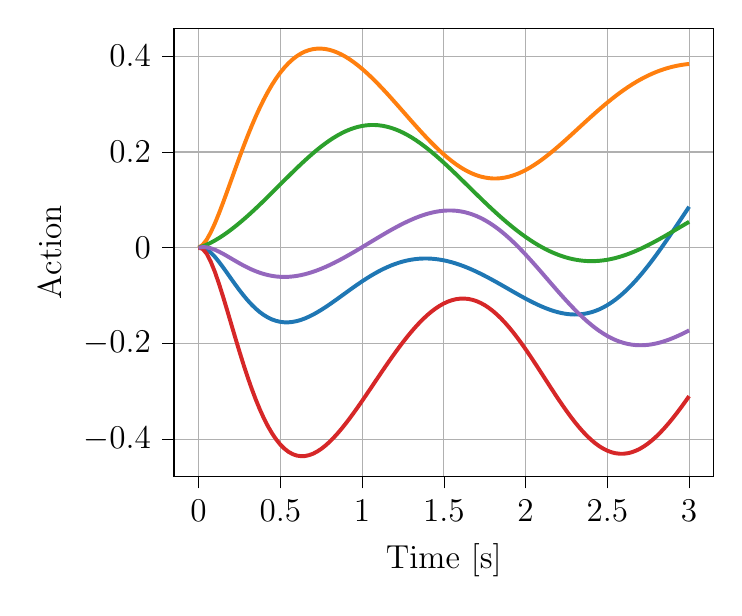
\begin{tikzpicture}
{
% \scriptsize
\fontsize{12}{12}\selectfont
\definecolor{crimson2143940}{RGB}{214,39,40}
\definecolor{darkgray176}{RGB}{176,176,176}
\definecolor{darkorange25512714}{RGB}{255,127,14}
\definecolor{forestgreen4416044}{RGB}{44,160,44}
\definecolor{mediumpurple148103189}{RGB}{148,103,189}
\definecolor{steelblue31119180}{RGB}{31,119,180}
\def\linewidth{0.5mm}
% This file was created with tikzplotlib v0.10.1.

\begin{axis}[
tick align=outside,
tick pos=left,
x grid style={darkgray176},
xlabel={Time [s]},
xmajorgrids,
xmin=-0.15, xmax=3.15,
xtick style={color=black},
y grid style={darkgray176},
% ylabel={Torque [N·m]},
ylabel={Action},
ymajorgrids,
ymin=-0.478080229461193, ymax=0.458539353311062,
ytick style={color=black}
]
\addplot [line width=\linewidth, steelblue31119180]
table {%
0 0
0.0250000022351742 0.000109076499938965
0.0500000044703484 -0.00352883338928223
0.0750000029802322 -0.0102730691432953
0.100000008940697 -0.0191351473331451
0.125 -0.0296087265014648
0.150000005960464 -0.0410379767417908
0.174999997019768 -0.0530241429805756
0.200000017881393 -0.0651566386222839
0.225000008940697 -0.0771229267120361
0.25 -0.0886918008327484
0.275000005960464 -0.0996206700801849
0.300000011920929 -0.109807312488556
0.324999988079071 -0.119066506624222
0.349999994039536 -0.127386718988419
0.375 -0.134629964828491
0.400000035762787 -0.140846699476242
0.425000011920929 -0.145938009023666
0.450000017881393 -0.149994850158691
0.474999994039536 -0.152951121330261
0.5 -0.154921531677246
0.524999976158142 -0.155866891145706
0.550000011920929 -0.155914098024368
0.575000047683716 -0.155046612024307
0.600000023841858 -0.153393894433975
0.625 -0.150958329439163
0.649999976158142 -0.147865206003189
0.675000011920929 -0.144132375717163
0.699999988079071 -0.139876544475555
0.725000023841858 -0.135127812623978
0.75 -0.129991322755814
0.774999976158142 -0.124506086111069
0.800000071525574 -0.118764042854309
0.825000047683716 -0.112810999155045
0.850000023841858 -0.106723546981812
0.875000059604645 -0.100553065538406
0.900000035762787 -0.0943605303764343
0.925000011920929 -0.0881997048854828
0.949999988079071 -0.0821165442466736
0.975000023841858 -0.0761667191982269
1 -0.0703805983066559
1.02499997615814 -0.0648128390312195
1.04999995231628 -0.0594816207885742
1.07500004768372 -0.0544395446777344
1.10000002384186 -0.0496918559074402
1.125 -0.0452891290187836
1.15000009536743 -0.0412254631519318
1.17500007152557 -0.0375468134880066
1.20000004768372 -0.0342386662960052
1.22500002384186 -0.0313448309898376
1.25 -0.0288401544094086
1.27500009536743 -0.0267651379108429
1.29999995231628 -0.0250891745090485
1.32500004768372 -0.0238471031188965
1.35000002384186 -0.0230042040348053
1.375 -0.0225905776023865
1.39999997615814 -0.0225684940814972
1.42500007152557 -0.0229629576206207
1.45000004768372 -0.0237343311309814
1.47500002384186 -0.0249029099941254
1.5 -0.0264270305633545
1.52499997615814 -0.0283234119415283
1.54999995231628 -0.030549943447113
1.57499992847443 -0.0331180393695831
1.59999990463257 -0.0359856188297272
1.62499988079071 -0.0391594767570496
1.65000009536743 -0.0425972938537598
1.67499995231628 -0.0463020801544189
1.70000004768372 -0.0502311587333679
1.72499990463257 -0.0543811619281769
1.75 -0.0587121844291687
1.77499985694885 -0.0632140636444092
1.79999995231628 -0.0678482353687286
1.82500004768372 -0.0725975036621094
1.85000002384186 -0.0774255096912384
1.875 -0.0823085606098175
1.89999997615814 -0.0872117578983307
1.92499995231628 -0.0921027958393097
1.94999992847443 -0.0969512760639191
1.97499990463257 -0.101717948913574
2 -0.106374353170395
2.02500009536743 -0.110872626304626
2.04999995231628 -0.115190327167511
2.07500004768372 -0.119272261857986
2.09999990463257 -0.123099237680435
2.125 -0.126610994338989
2.14999985694885 -0.129795491695404
2.17499995231628 -0.132583230733871
2.20000004768372 -0.134972095489502
2.22499990463257 -0.13688912987709
2.25 -0.138336986303329
2.27500009536743 -0.139243394136429
2.29999995231628 -0.13961997628212
2.32499980926514 -0.13939180970192
2.34999990463257 -0.138581871986389
2.375 -0.137117832899094
2.40000009536743 -0.135032713413239
2.42499995231628 -0.132259339094162
2.45000004768372 -0.128839164972305
2.47499990463257 -0.124712765216827
2.5 -0.119931876659393
2.52499985694885 -0.114445954561234
2.55000019073486 -0.108314603567123
2.57500004768372 -0.101498186588287
2.59999990463257 -0.094064474105835
2.625 -0.0859843194484711
2.65000009536743 -0.0773324072360992
2.67499995231628 -0.0680895149707794
2.69999980926514 -0.0583319962024689
2.72499990463257 -0.0480563640594482
2.75 -0.0373404026031494
2.77500009536743 -0.0261877477169037
2.79999995231628 -0.01467365026474
2.82500004768372 -0.00281539559364319
2.84999990463257 0.00931799411773682
2.875 0.0216982960700989
2.89999985694885 0.0342642068862915
2.92500019073486 0.0469831824302673
2.95000004768372 0.0597984194755554
2.97499990463257 0.072671115398407
3 0.0855525732040405
};
\addplot [line width=\linewidth, darkorange25512714]
table {%
0 0
0.0250000022351742 0.00577962398529053
0.0500000044703484 0.0168243050575256
0.0750000029802322 0.0322830080986023
0.100000008940697 0.050804078578949
0.125 0.0717223882675171
0.150000005960464 0.0941377878189087
0.174999997019768 0.117531001567841
0.200000017881393 0.141331970691681
0.225000008940697 0.165135860443115
0.25 0.188610672950745
0.275000005960464 0.211441218852997
0.300000011920929 0.233464539051056
0.324999988079071 0.254435420036316
0.349999994039536 0.274309098720551
0.375 0.292894423007965
0.400000035762787 0.310226082801819
0.425000011920929 0.326155781745911
0.450000017881393 0.340769410133362
0.474999994039536 0.353951156139374
0.5 0.365818500518799
0.524999976158142 0.376281440258026
0.550000011920929 0.385473191738129
0.575000047683716 0.393323600292206
0.600000023841858 0.399972558021545
0.625 0.405364632606506
0.649999976158142 0.409639537334442
0.675000011920929 0.412753283977509
0.699999988079071 0.414841830730438
0.725000023841858 0.415869891643524
0.75 0.415965735912323
0.774999976158142 0.415102481842041
0.800000071525574 0.413399219512939
0.825000047683716 0.410836398601532
0.850000023841858 0.407524228096008
0.875000059604645 0.403448522090912
0.900000035762787 0.398711681365967
0.925000011920929 0.393305122852325
0.949999988079071 0.387323558330536
0.975000023841858 0.380764305591583
1 0.373714447021484
1.02499997615814 0.366179287433624
1.04999995231628 0.358237445354462
1.07500004768372 0.349901854991913
1.10000002384186 0.341244876384735
1.125 0.332286655902863
1.15000009536743 0.323093235492706
1.17500007152557 0.31369411945343
1.20000004768372 0.304148137569427
1.22500002384186 0.294490873813629
1.25 0.284777641296387
1.27500009536743 0.275051057338715
1.29999995231628 0.265359044075012
1.32500004768372 0.255752384662628
1.35000002384186 0.246270954608917
1.375 0.236973226070404
1.39999997615814 0.227889716625214
1.42500007152557 0.219086170196533
1.45000004768372 0.2105832695961
1.47500002384186 0.202451646327972
1.5 0.194703161716461
1.52499997615814 0.187410295009613
1.54999995231628 0.180574715137482
1.57499992847443 0.174270570278168
1.59999990463257 0.168488323688507
1.62499988079071 0.163301587104797
1.65000009536743 0.158690273761749
1.67499995231628 0.154723823070526
1.70000004768372 0.151371717453003
1.72499990463257 0.148699760437012
1.75 0.146665751934052
1.77499985694885 0.145328283309937
1.79999995231628 0.144636154174805
1.82500004768372 0.144640803337097
1.85000002384186 0.145281493663788
1.875 0.14659970998764
1.89999997615814 0.148529529571533
1.92499995231628 0.151102602481842
1.94999992847443 0.154246985912323
1.97499990463257 0.1579829454422
2 0.162237584590912
2.02500009536743 0.167022526264191
2.04999995231628 0.172261714935303
2.07500004768372 0.177957773208618
2.09999990463257 0.18403834104538
2.125 0.190493583679199
2.14999985694885 0.197255313396454
2.17499995231628 0.204309463500977
2.20000004768372 0.211590230464935
2.22499990463257 0.219075441360474
2.25 0.226709604263306
2.27500009536743 0.23446124792099
2.29999995231628 0.24228447675705
2.32499980926514 0.250144481658936
2.34999990463257 0.258001685142517
2.375 0.265819489955902
2.40000009536743 0.27356630563736
2.42499995231628 0.281202137470245
2.45000004768372 0.288708031177521
2.47499990463257 0.296041190624237
2.5 0.303189754486084
2.52499985694885 0.310113847255707
2.55000019073486 0.316808640956879
2.57500004768372 0.323233783245087
2.59999990463257 0.329395115375519
2.625 0.33525276184082
2.65000009536743 0.34081643819809
2.67499995231628 0.346053123474121
2.69999980926514 0.350978553295135
2.72499990463257 0.355558693408966
2.75 0.359813511371613
2.77500009536743 0.363716781139374
2.79999995231628 0.367293477058411
2.82500004768372 0.370514869689941
2.84999990463257 0.373411655426025
2.875 0.37595921754837
2.89999985694885 0.378187835216522
2.92500019073486 0.380078911781311
2.95000004768372 0.381663918495178
2.97499990463257 0.382924258708954
3 0.383891403675079
};
\addplot [line width=\linewidth, forestgreen4416044]
table {%
0 0
0.0250000022351742 0.00284212827682495
0.0500000044703484 0.00632262229919434
0.0750000029802322 0.01042240858078
0.100000008940697 0.0150365829467773
0.125 0.020155131816864
0.150000005960464 0.025696873664856
0.174999997019768 0.0316569805145264
0.200000017881393 0.0379704833030701
0.225000008940697 0.0446345210075378
0.25 0.0515945553779602
0.275000005960464 0.0588470697402954
0.300000011920929 0.0663439035415649
0.324999988079071 0.0740782022476196
0.349999994039536 0.0820066332817078
0.375 0.0901170969009399
0.400000035762787 0.0983688235282898
0.425000011920929 0.106744110584259
0.450000017881393 0.115204274654388
0.474999994039536 0.123723804950714
0.5 0.13226717710495
0.524999976158142 0.140801727771759
0.550000011920929 0.149294376373291
0.575000047683716 0.157705247402191
0.600000023841858 0.16600501537323
0.625 0.17414653301239
0.649999976158142 0.182106196880341
0.675000011920929 0.189829885959625
0.699999988079071 0.197300553321838
0.725000023841858 0.20445853471756
0.75 0.211293876171112
0.774999976158142 0.217743694782257
0.800000071525574 0.223804950714111
0.825000047683716 0.229413330554962
0.850000023841858 0.234574794769287
0.875000059604645 0.239223301410675
0.900000035762787 0.243374466896057
0.925000011920929 0.246963918209076
0.949999988079071 0.250016450881958
0.975000023841858 0.252469658851624
1 0.254358172416687
1.02499997615814 0.255625128746033
1.04999995231628 0.25631183385849
1.07500004768372 0.256367862224579
1.10000002384186 0.255842566490173
1.125 0.254692018032074
1.15000009536743 0.252971529960632
1.17500007152557 0.250647068023682
1.20000004768372 0.24777740240097
1.22500002384186 0.244334638118744
1.25 0.240383923053741
1.27500009536743 0.235904932022095
1.29999995231628 0.230963170528412
1.32500004768372 0.225547730922699
1.35000002384186 0.219722926616669
1.375 0.21348625421524
1.39999997615814 0.206899642944336
1.42500007152557 0.199968338012695
1.45000004768372 0.192750215530396
1.47500002384186 0.185257494449615
1.5 0.177544295787811
1.52499997615814 0.169627130031586
1.54999995231628 0.161554396152496
1.57499992847443 0.15334814786911
1.59999990463257 0.145050764083862
1.62499988079071 0.136687636375427
1.65000009536743 0.128295242786407
1.67499995231628 0.11990088224411
1.70000004768372 0.111534774303436
1.72499990463257 0.103228032588959
1.75 0.095002293586731
1.77499985694885 0.0868906378746033
1.79999995231628 0.0789086222648621
1.82500004768372 0.0710912942886353
1.85000002384186 0.063447117805481
1.875 0.0560116171836853
1.89999997615814 0.0487884879112244
1.92499995231628 0.041814923286438
1.94999992847443 0.0350876450538635
1.97499990463257 0.028643786907196
2 0.0224764347076416
2.02500009536743 0.0166246891021729
2.04999995231628 0.0110754370689392
2.07500004768372 0.00586789846420288
2.09999990463257 0.000986933708190918
2.125 -0.0035298764705658
2.14999985694885 -0.00770196318626404
2.17499995231628 -0.0114883482456207
2.20000004768372 -0.0149144232273102
2.22499990463257 -0.0179407000541687
2.25 -0.0205923616886139
2.27500009536743 -0.0228343307971954
2.29999995231628 -0.0246939957141876
2.32499980926514 -0.0261361002922058
2.34999990463257 -0.0271928608417511
2.375 -0.027831643819809
2.40000009536743 -0.0280870497226715
2.42499995231628 -0.02793088555336
2.45000004768372 -0.0273983478546143
2.47499990463257 -0.0264663100242615
2.5 -0.0251731276512146
2.52499985694885 -0.0234997272491455
2.55000019073486 -0.0214857459068298
2.57500004768372 -0.0191183984279633
2.59999990463257 -0.0164380967617035
2.625 -0.0134372115135193
2.65000009536743 -0.0101584494113922
2.67499995231628 -0.00659698247909546
2.69999980926514 -0.0027942955493927
2.72499990463257 0.00124549865722656
2.75 0.005482017993927
2.77500009536743 0.00991016626358032
2.79999995231628 0.0144922137260437
2.82500004768372 0.0192152261734009
2.84999990463257 0.0240467190742493
2.875 0.0289692282676697
2.89999985694885 0.0339543223381042
2.92500019073486 0.0389840006828308
2.95000004768372 0.0440326333045959
2.97499990463257 0.0490788817405701
3 0.0541011691093445
};
\addplot [line width=\linewidth, crimson2143940]
table {%
0 0
0.0250000022351742 -0.00241938233375549
0.0500000044703484 -0.0126208364963531
0.0750000029802322 -0.0293452143669128
0.100000008940697 -0.0505895614624023
0.125 -0.0753616690635681
0.150000005960464 -0.102322578430176
0.174999997019768 -0.130691945552826
0.200000017881393 -0.159619480371475
0.225000008940697 -0.188492774963379
0.25 -0.216817617416382
0.275000005960464 -0.244115769863129
0.300000011920929 -0.270148456096649
0.324999988079071 -0.294544875621796
0.349999994039536 -0.317245602607727
0.375 -0.33796638250351
0.400000035762787 -0.356770515441895
0.425000011920929 -0.373442888259888
0.450000017881393 -0.388127446174622
0.474999994039536 -0.40066534280777
0.5 -0.411249250173569
0.524999976158142 -0.419765055179596
0.550000011920929 -0.426431685686111
0.575000047683716 -0.431171536445618
0.600000023841858 -0.434212565422058
0.625 -0.435506612062454
0.649999976158142 -0.435278922319412
0.675000011920929 -0.433504968881607
0.699999988079071 -0.430399775505066
0.725000023841858 -0.425957649946213
0.75 -0.420378148555756
0.774999976158142 -0.413670599460602
0.800000071525574 -0.406016558408737
0.825000047683716 -0.397437989711761
0.850000023841858 -0.388096570968628
0.875000059604645 -0.378024578094482
0.900000035762787 -0.367364108562469
0.925000011920929 -0.356156051158905
0.949999988079071 -0.344523131847382
0.975000023841858 -0.332515180110931
1 -0.320235431194305
1.02499997615814 -0.30774050951004
1.04999995231628 -0.295117855072021
1.07500004768372 -0.282430648803711
1.10000002384186 -0.269749730825424
1.125 -0.257145822048187
1.15000009536743 -0.244674742221832
1.17500007152557 -0.232412129640579
1.20000004768372 -0.220400899648666
1.22500002384186 -0.208725214004517
1.25 -0.197411507368088
1.27500009536743 -0.186550587415695
1.29999995231628 -0.176158100366592
1.32500004768372 -0.166327834129333
1.35000002384186 -0.157064497470856
1.375 -0.1484654545784
1.39999997615814 -0.140525013208389
1.42500007152557 -0.133341819047928
1.45000004768372 -0.126898646354675
1.47500002384186 -0.121295958757401
1.5 -0.116502702236176
1.52499997615814 -0.112620502710342
1.54999995231628 -0.10960641503334
1.57499992847443 -0.107556968927383
1.59999990463257 -0.10641747713089
1.62499988079071 -0.106279402971268
1.65000009536743 -0.107074290513992
1.67499995231628 -0.10888734459877
1.70000004768372 -0.111635684967041
1.72499990463257 -0.115392476320267
1.75 -0.120066165924072
1.77499985694885 -0.125713706016541
1.79999995231628 -0.132234692573547
1.82500004768372 -0.139668226242065
1.85000002384186 -0.147905975580215
1.875 -0.15696969628334
1.89999997615814 -0.166744530200958
1.92499995231628 -0.177229195833206
1.94999992847443 -0.188309520483017
1.97499990463257 -0.199964076280594
2 -0.212077170610428
2.02500009536743 -0.224605441093445
2.04999995231628 -0.237438797950745
2.07500004768372 -0.250514447689056
2.09999990463257 -0.263727486133575
2.125 -0.276997566223145
2.14999985694885 -0.290233373641968
2.17499995231628 -0.303332567214966
2.20000004768372 -0.316223084926605
2.22499990463257 -0.328789949417114
2.25 -0.34097284078598
2.27500009536743 -0.352651655673981
2.29999995231628 -0.363786607980728
2.32499980926514 -0.374247878789902
2.34999990463257 -0.384018272161484
2.375 -0.392969578504562
2.40000009536743 -0.401105284690857
2.42499995231628 -0.408300429582596
2.45000004768372 -0.414580345153809
2.47499990463257 -0.419827491044998
2.5 -0.424089521169662
2.52499985694885 -0.427261859178543
2.55000019073486 -0.429409116506577
2.57500004768372 -0.430440753698349
2.59999990463257 -0.430442631244659
2.625 -0.429337799549103
2.65000009536743 -0.427227109670639
2.67499995231628 -0.424050718545914
2.69999980926514 -0.419917166233063
2.72499990463257 -0.414788544178009
2.75 -0.408781945705414
2.77500009536743 -0.401871085166931
2.79999995231628 -0.394175887107849
2.82500004768372 -0.385688662528992
2.84999990463257 -0.376525193452835
2.875 -0.366696059703827
2.89999985694885 -0.356308937072754
2.92500019073486 -0.345382839441299
2.95000004768372 -0.334022760391235
2.97499990463257 -0.322257429361343
3 -0.310181736946106
};
\addplot [line width=\linewidth, mediumpurple148103189]
table {%
0 0
0.0250000022351742 0.00132888555526733
0.0500000044703484 0.000835120677947998
0.0750000029802322 -0.00119742751121521
0.100000008940697 -0.00430575013160706
0.125 -0.00826326012611389
0.150000005960464 -0.0127565264701843
0.174999997019768 -0.0176048576831818
0.200000017881393 -0.0226060748100281
0.225000008940697 -0.027616024017334
0.25 -0.0325145721435547
0.275000005960464 -0.0371871888637543
0.300000011920929 -0.0415735244750977
0.324999988079071 -0.0455831587314606
0.349999994039536 -0.0491979122161865
0.375 -0.0523473620414734
0.400000035762787 -0.0550429224967957
0.425000011920929 -0.0572300851345062
0.450000017881393 -0.058940201997757
0.474999994039536 -0.0601321756839752
0.5 -0.060849666595459
0.524999976158142 -0.0610618591308594
0.550000011920929 -0.0608198642730713
0.575000047683716 -0.0601015090942383
0.600000023841858 -0.0589609146118164
0.625 -0.0573831498622894
0.649999976158142 -0.0554222166538239
0.675000011920929 -0.0530692040920258
0.699999988079071 -0.0503761768341064
0.725000023841858 -0.0473393797874451
0.75 -0.0440076291561127
0.774999976158142 -0.0403813719749451
0.800000071525574 -0.0365063548088074
0.825000047683716 -0.0323863923549652
0.850000023841858 -0.0280632078647614
0.875000059604645 -0.0235447883605957
0.900000035762787 -0.0188689231872559
0.925000011920929 -0.0140470564365387
0.949999988079071 -0.00911316275596619
0.975000023841858 -0.0040835440158844
1 0.00101196765899658
1.02499997615814 0.00615376234054565
1.04999995231628 0.0113139152526855
1.07500004768372 0.0164682269096375
1.10000002384186 0.0215928554534912
1.125 0.0266581773757935
1.15000009536743 0.0316434502601624
1.17500007152557 0.0365153551101685
1.20000004768372 0.0412558913230896
1.22500002384186 0.0458242297172546
1.25 0.0502094626426697
1.27500009536743 0.0543646812438965
1.29999995231628 0.0582819581031799
1.32500004768372 0.0619113445281982
1.35000002384186 0.0652486085891724
1.375 0.0682399272918701
1.39999997615814 0.0708852410316467
1.42500007152557 0.073128879070282
1.45000004768372 0.0749759674072266
1.47500002384186 0.0763683915138245
1.5 0.0773192048072815
1.52499997615814 0.0777676701545715
1.54999995231628 0.0777335166931152
1.57499992847443 0.0771585702896118
1.59999990463257 0.076069176197052
1.62499988079071 0.0744092464447021
1.65000009536743 0.0722140669822693
1.67499995231628 0.0694298148155212
1.70000004768372 0.0661012530326843
1.72499990463257 0.0621816515922546
1.75 0.0577211976051331
1.77499985694885 0.0526820421218872
1.79999995231628 0.0471206307411194
1.82500004768372 0.0410100817680359
1.85000002384186 0.0344118475914001
1.875 0.0273085832595825
1.89999997615814 0.0197672247886658
1.92499995231628 0.0117847323417664
1.94999992847443 0.00342720746994019
1.97499990463257 -0.00529712438583374
2 -0.0143193602561951
2.02500009536743 -0.0236175060272217
2.04999995231628 -0.0331268608570099
2.07500004768372 -0.0428137183189392
2.09999990463257 -0.0526146292686462
2.125 -0.0624864995479584
2.14999985694885 -0.0723739564418793
2.17499995231628 -0.0822190642356873
2.20000004768372 -0.0919783413410187
2.22499990463257 -0.101586788892746
2.25 -0.111006081104279
2.27500009536743 -0.120169281959534
2.29999995231628 -0.129049569368362
2.32499980926514 -0.137572884559631
2.34999990463257 -0.145726323127747
2.375 -0.153436571359634
2.40000009536743 -0.160702258348465
2.42499995231628 -0.16745188832283
2.45000004768372 -0.173695653676987
2.47499990463257 -0.179366737604141
2.5 -0.184488445520401
2.52499985694885 -0.189000338315964
2.55000019073486 -0.192935973405838
2.57500004768372 -0.196242570877075
2.59999990463257 -0.198965460062027
2.625 -0.2010597884655
2.65000009536743 -0.202580541372299
2.67499995231628 -0.20349046587944
2.69999980926514 -0.20384955406189
2.72499990463257 -0.203634172677994
2.75 -0.202909767627716
2.77500009536743 -0.201656997203827
2.79999995231628 -0.199943691492081
2.82500004768372 -0.19776263833046
2.84999990463257 -0.195178627967834
2.875 -0.192194640636444
2.89999985694885 -0.188872009515762
2.92500019073486 -0.185217648744583
2.95000004768372 -0.181291848421097
2.97499990463257 -0.177107751369476
3 -0.172720789909363
};
\end{axis}
}
\end{tikzpicture}
}%
    %     }
    %     \captionsetup{margin={7.5mm,0mm}}
    %     \caption{}
    %     \label{subfig:mp_traj}
    % \end{subfigure}        